\documentclass[a4paper,12pt]{report}
\usepackage[T1]{fontenc}
\usepackage[utf8]{inputenc}
\usepackage[italian]{babel}
\usepackage{microtype}
\usepackage{lmodern}
\renewcommand{\thefootnote}{\fnsymbol{footnote}}
\usepackage{listings}
\usepackage{graphicx}
\usepackage{rotating}
\usepackage[italian]{varioref}
\usepackage{caption}
\captionsetup{tableposition=top,figureposition=bottom,font=small,format=hang,labelfont={sf,bf}}
\usepackage{float}
\usepackage{listings}
\usepackage[dvipsnames]{xcolor}
\usepackage{color}
\newcommand{\mychapter}[2]{
	\setcounter{chapter}{#1}
	\setcounter{section}{0}
	\chapter*{#2}
	\addcontentsline{toc}{chapter}{#2}
}

\definecolor{deepblue}{rgb}{0,0,0.5}
\definecolor{deepred}{rgb}{0.6,0,0}
\definecolor{deepgreen}{rgb}{0,0.5,0}
\definecolor{light-gray}{gray}{0.90}
\DeclareFixedFont{\ttb}{T1}{txtt}{bx}{n}{12} % for bold
\DeclareFixedFont{\ttm}{T1}{txtt}{m}{n}{12}  % for normal


\newcommand\realnumberstyle[1]{}


% Python style for highlighting
\newcommand\pythonstyle{\lstset{
		language=Python,
		basicstyle=\ttm,
		otherkeywords={self},             % Add keywords here
		keywordstyle=\ttb\color{deepblue},
		emph={MyClass,__init__},          % Custom highlighting
		emphstyle=\ttb\color{deepred},    % Custom highlighting style
		stringstyle=\color{deepgreen},
		frame=tb,                         % Any extra options here
		showstringspaces=false 
		xleftmargin=\dimexpr\fboxsep-\fboxrule,
		xrightmargin=\dimexpr\fboxsep-\fboxrule,
		gobble=16 ,
		numbers=left
	}}
	
	
	% Python environment
	\lstnewenvironment{python}[1][]
	{
		\pythonstyle
		\lstset{#1}
	}
	{}
\begin{document}        
	\begin{titlepage}
		\centering
		{\scshape\huge Università degli Studi di Napoli Federico II \par}
		\vspace{1cm}
		{\scshape\large Dipartimento di Ingegneria Elettrica e delle Tecnologie dell'Informazione\par}
		\vspace{0.5cm}
		{\scshape\large Corso di Intelligenza Artificiale\par}
		\vspace{1.5cm}
		{\ttfamily\Large Elaborato Esercitativo\par}
		\vspace{0.5cm}
		{\huge\bfseries Work Projects\par}
		\vspace{2cm}
		{\Large\itshape Milo Saverio\par}
		{\Large\itshape Previtera Gabriele\par}
		{\Large\itshape Pommella Michele\par}
		\vspace{1.5cm}
		{\large Prof.~Neri Filippo\par}
		
		\vfill
		
		% Bottom of the page
		{\large Anno 2016-2017\par}
		
		%\definecolor{deepblue}{rgb}{0,0,0.5}
\definecolor{deepred}{rgb}{0.6,0,0}
\definecolor{deepgreen}{rgb}{0,0.5,0}
\DeclareFixedFont{\ttb}{T1}{txtt}{bx}{n}{12} % for bold
\DeclareFixedFont{\ttm}{T1}{txtt}{m}{n}{12}  % for normal


\newcommand\realnumberstyle[1]{}


% Python style for highlighting
\newcommand\pythonstyle{\lstset{
		language=Python,
		basicstyle=\ttm,
		otherkeywords={self},             % Add keywords here
		keywordstyle=\ttb\color{deepblue},
		emph={MyClass,__init__},          % Custom highlighting
		emphstyle=\ttb\color{deepred},    % Custom highlighting style
		stringstyle=\color{deepgreen},
		frame=tb,                         % Any extra options here
		showstringspaces=false 
		xleftmargin=\dimexpr\fboxsep-\fboxrule,
		xrightmargin=\dimexpr\fboxsep-\fboxrule,
		gobble=16 ,
		numbers=left
	}}
	
	
	% Python environment
	\lstnewenvironment{python}[1][]
	{
		\pythonstyle
		\lstset{#1}
	}
	{}

\mychapter{1}{Decision Trees}
	\label{ch:dt}
	Questo primo lavoro di gruppo si incentra sulla comprensione empirica dei \textsf{Decision Trees}, esempio di strumento ampiamente diffuso nel \textsf{ Machine Learning}, e sul \textsf{Problem Solving}, metodo scientifico applicato dall'\textsf{I.A.} per la risoluzione dei problemi.
	\section{Esercizio 1}
		\label{sec:es1}
		\subsection{}
		
		%io non direi grafo a finale un albero e' una sorta di specializzazione di un grafo
		Un albero di decisione è un grafo delle decisioni e delle loro possibili conseguenze, costruito al fine di supportare l'azione decisionale. Rappresenta un importante strumento nel contesto dell'\textsf{Inductive Learning}, in cui ricopre il ruolo di modello predittivo su cui si basa il comportamento dell'agente.\newline La sua struttura discende da un insieme di esempi dati e determina le regole di condizione-azione atte alla classificazione di esempi futuri.%parlerei anche di bonta' dell'apprendimento dicendo che se dai piu' dat apprende di piu'  e blablabla
		 Dunque l'agente è in grado di apprendere da una serie di dati il comportamento da assumere in situazioni non specificate.
		
		Come primo esperimento abbiamo adoperato un insieme di dati facenti riferimento a vari tipi di \emph{Iris}, caratterizzati da quattro attributi.
		%\begin{itemize}
		%	\item lunghezza del sepalo
		%	\item larghezza del sepalo
		%	\item lunghezza del petalo
		%	\item larghezza del petalo
		%\end{itemize}
		Queste grandezze sono dimensionalmente espresse tutte in cm. La dimensione complessiva del dataset è di 150 elementi. Per effettuare la prova è stato necessario formattare l'insieme dei dati originario, rendendolo consistente con le esigenze algoritmiche correlate al linguaggio utilizzato, \emph{Python} nel nostro caso.\newline Gli esempi del dataset si presentano nella forma:
		\lstinputlisting[lastline=1]{iris.txt}
		Abbiamo, dunque, determinato i valori di ciascun esempio attraverso le virgole delimitatorie, riconosciuto i valori numerici (precedentemente visti come stringhe) definendoli come tali ed eliminato eventualmente il carattere di \textit{new line} al fine di evitare valori spuri.
		\medskip
		\begin{python}
		def aprifile(fil="nomefile.txt"):
			data=[]
			for line in file(fil):
				srt=line.split(',')
				for count in range(0,len(srt)):
					if(isfloat(srt[count])):
						srt[count]=float(srt[count])
					else :
						srt[count]=srt[count].strip('\n')
				data=data+[srt];
			return data
		\end{python}
		\bigskip
		Un campione di esempio formattato si presenterà, dunque, nella forma:
		\lstinputlisting[lastline=1]{irisformattato.txt}

		
		Decidiamo di usare il 40\% dei dati forniti dal dataset per il training, quindi per l' apprendimento, ed un 60 \% per il test.
		Per la determinazione di training set e test set si è utilizzata una funzione che selezioni un insieme casuale di esempi dal data set di partenza, con cardinalità determinata dai parametri di ingresso.
		\bigskip
		\begin{python}
		def createdataset(data,numdati):
			tr=[]
			te=[]
			t=[]
			for i in range(0,numdati):
				t=random.choice(data);
				tr=tr+[t]
				num=data.index(t)
				del data[num]
			te=data
			return(tr,te)
		\end{python}
		Decidiamo di usare un 
		40\% per il training, quindi per l' apprendimento, ed un 60 \% per il test.
		%espresse in cm.La dimensione complessiva del dataset che abbiamo utilizzato e' di 150 elementi. Nel primo test del codice che abbiamo effettuato abbiamo deciso di utilizzare il ... tali set di dati sono costruiti automaticamente da una funzione da noi scritta che crea i data set scegliendo elementi random
		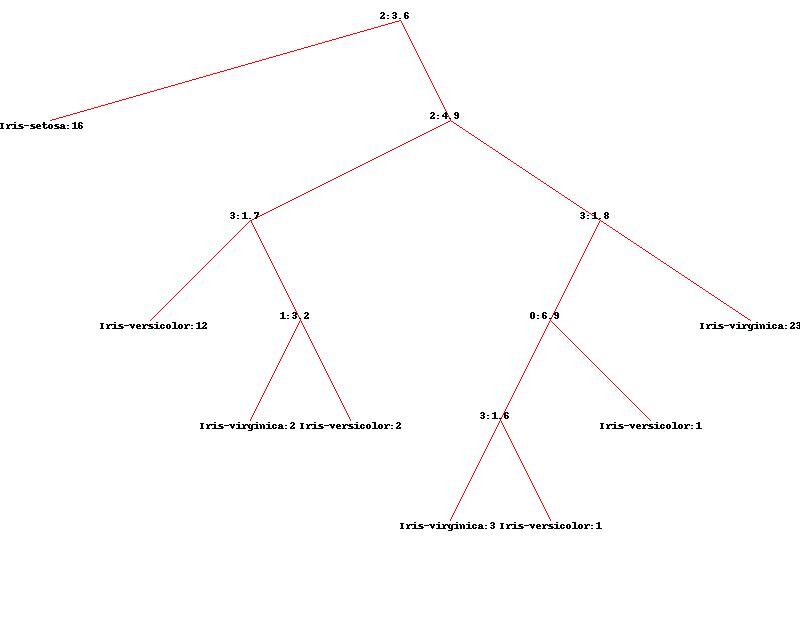
\includegraphics[scale=0.37]{iris.jpg}
		
		 Come si evince dalla figura, il nodo scelto come radice è la terza colonna(colonna numero 2 da programma, perché la numerazione effettuata dal codice della classificazione rimarca quella delle liste in python) ed il valore che  minimizza la funzione d' entropia è 3.6, infatti ci permette di caratterizzare già 16 esempi.
		  L'albero con le informazioni di training, riesce a classificare tutti gli esempi, anche se il contenuto informativo degli attribbuti non è alto, perché come vediamo, un attributo non riesce a caratterizzare nettamente un gruppo di esempi.Infatti più volte sono richiamati gli stessi attribbuti per splittare nuovamente i dati, aumentando così la profondità dell' albero. \newline Quest' ultimo,per tale ragione non può essere considerato generico, molto probabilmente se utlizziamo per il test un test-set contenete dati molto diversi da quelli con cui è stato effettuato il training non ci offrira' ottimi risultati. 
		  \newline Una soluzione a tale problema potrebbe essere l'applicazione di una potatura su alcuni rami, in modo tale da renderlo più semplice.
		  \newline Tale soluzione ha come fondamenta l'enunciato di Okam, anche conosciuto come  \textbf{\textit{rasoio di Okam}}.
		\newline
		\newline
		%li separeri come paragrafo uno chiamerei iris e uno fughi 
		Ora invece ci concentriamo su un diverso dataset relativo ai funghi,scopo ultimo di questo dataset è determinare l' habitat in cui i funghi vivono.Il dataset è caratterizzato da ben 22 attributi, utilizziamo sempre la stessa percentuali di dati per il training ed il test set.
		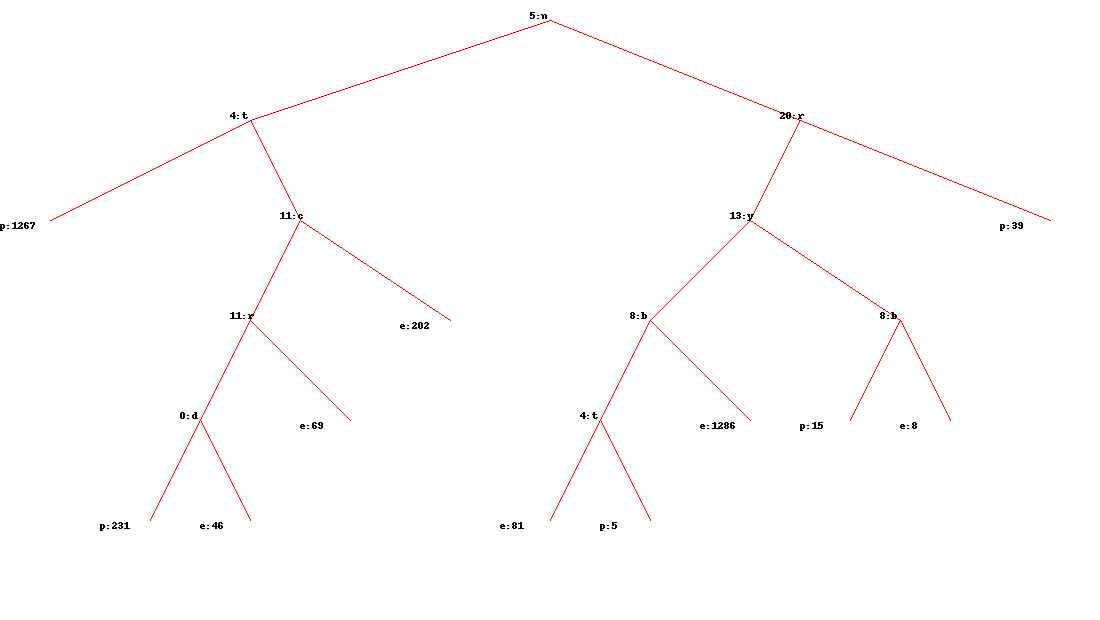
\includegraphics[width=.9\textwidth, height=0.63\textheight]{mushroom.jpg}		
		\newline L' albero,come si può osservare non è in grado di classificare gli esempi distintamente.
		%in seguito a vari test effettuati con diversi elementi che componevano il training set, i risultati sono appartsi sempre inconcludenti in quanto c'era sempre un numero di nodi maggiore di 3 che portavano a decisioni ambuigue, nel nodo foglia c'erano piu' risultati.Per tanto visto che stiamo studiando tale materia abbiamo deciso di soffermarci su tali risultati giungendo alle seguenti conclusioni enumerato quello che sta dopo. 
	    Tale risultato può essere conseguenza dal fatto che il numero di esempi usato per il training sia troppo piccolo, quindi non capace di permettere di discriminare appieno una scelta, oppure gli attributi utilizzati non sono abbastanza rappresentativi, non riuscendo a classificare appieno i vari esempi, quindi bisognerebbe introdurre altri attributi oppure modificare quelli usati,in questo stato l' albero può portare a decisioni includenti.
	    Come si può osservare dai 2 esempi di data set, un alto numero di attributi, non è detto che ci porti a spiegare tutti gli esempi, infatti l' albero relativo ai funghi non utilizza tutte le caratteristiche ma solo alcune, quelle con un contenuto informativo più alto, abolendo le altre, però l' albero dei funghi molto probabilmente riuscirà a darci buoni risultati anche con casi sconosciuti essendo molto generico, quello degli iris no.
		\subsection{}
		In questo esempio mostreremo al variare del training set e del data set il cambiamento valore della performance dell' albero visualizzando tramite un grafico.
		Il data set che andremo ad utilizzare è stato preso da un censimento, per identificare le persone che guadagnano più di cinquanta mila dollari all' anno.
		Le righe di codice adibite alla generazione del grafico sono quelle scritte in questa funzione:
		\begin{python}
		def fperformance(data):
			testc=data
			percent=10
			p=[]
			perc=[]
			t=[]
			numdati=(int)((float)(len(testc))/100*percent);
			for i in range(0,5):
				(train,testc)=createdataset(testc,numdati)
				t=t+train;
				tree=buildtree(t)
				p=p+[performance(tree,testc)]
				perc=perc+[percent]
				percent=percent+10;
				line,=plt.plot(perc,p,'r-')
			plt.xlabel('percentuale dati training')
			plt.ylabel('percentuale successi')
			line.set_antialiased(False)
			plt.show()
		\end{python}
	%passiamo ora a descrivere cosa fa questa funzione come prima cosa effettua una copia del dataset che gli e' stato ricevuto dopodiche' inizializza una serie di liste a supporto delle operazioni successive. farei una descrizione per linee di codice, metterei il codice per riga sia sopra che sotto commentando
		la funzione essenzialmente dopo aver fatto una copia dei dati passati, fatto un paio di inizializzazione di liste che ci occorrono per il plot dei dati e aver determinato il numero di elementi da aggiungere al training set(togliendoli al test set), iterativamente per 5 volte divide i dati in train set e test set, dopo di che il train viene assegnata ad una lista t che incrementa ad ogni variazione e scritta su file da createdataset, viene costruito l' albero, se ne calcola il valore di performance, richiamando al suo interno la funzione classify che ritorna la classificazione  fatta dall ' albero con gli attributi dell' esempio e confrontandoli con il valore del test, se l' albero è riuscito a classificare bene l' esempio allora si avrà un riscontro positivo, altrimenti negativo, alla fine performance ritorna la percentuale di positivi sul numero di test effettuati.Dopo di che si aggiungono i punti alla linea per il plot e alla fine viene mostrata su schermo, un esempio di curva è questo:
		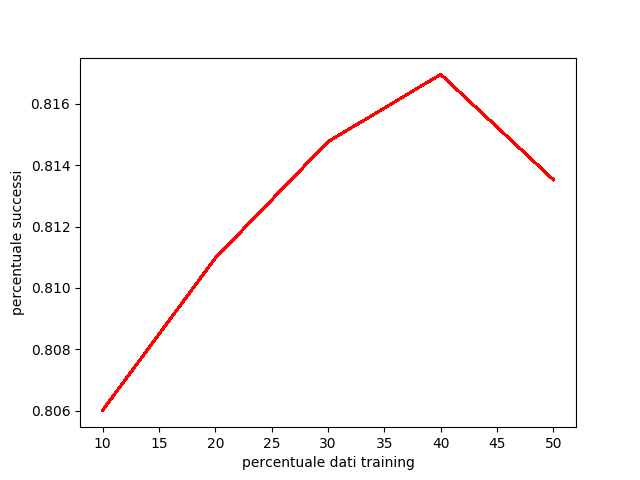
\includegraphics[scale=0.86]{performance.png}
		%evince 
		Come si vede dal grafico la nostra percentuale di apprendimento migliora fino al 40\% dopodiché si percepisce un degrado dell'apprendimento quando arriviamo al 50\% di dati utilizzati per il training-set.
		\newline
		 Su tale risultato siamo giunti alla seguente considerazione " aumentando il training-set si è costruito un albero più specifico e di conseguenza  con meno capacità di classificare gli esempi ".
		 Dalla figura che mostra l'andamento della curva di apprendimento, si intuisce che la rappresentazione dell'ambiente così descritto dai dataset è ridondante.
		  Infatti la crescita è lenta, al crescere del training-set dal 10\% al 50\% si evince che l'aumento è di circa del 1\%.
		  Per migliorare la rapidità della curva di performance dell'albero di decisione si potrebbero rimuovere alcuni attributi,se si è sicuri della rappresentazione, testando altre configurazioni dell' ambiente fino a che non vediamo miglioramenti evidenti nell' apprendimento, se ciò non avviene si può pensare di cambiare gli attributi che pensiamo ridondati o quelli che ci danno un basso contenuto informativo, con altri o addirittura rifare il modello dell' ambiente . 
		\subsection{}
		
		%tali tecniche di apprendimento mirano alla formulazione di una funzione h che approssimi la funzione f, dove ricordiamo che f è la funzione condizione azione che si vorrebbe apprendere. la costruione di h avviene 
			Un agente in grado di apprendere mediante alberi di decisione fonda questo suo processo su principi di apprendimento induttivo (\textsf{inductive learning}). L'apprendimento induttivo è una forma di apprendimento basata sull'induzione a partire da esempi dati. Esso, data una collezione di esempi (\textsf{training set}) della funzione \textsf{target} \emph{f} che si vorrebbe imparare, mira a restituire una funzione \emph{h} (\textsf{hypothesis}) che approssimi la \emph{f}, anche se non è detto che riesca a trovare una che l' approssimi bene nello spazio delle funzioni. Concettualmente, il criterio nella determinazione di \emph{h} tra le differenti funzioni dello spazio delle ipotesi dovrebbe essere legato, più che alla consistenza nello spiegare i dati, alla bontà dell'approssimazione e quindi alla capacità di generalizzazione per predire esempi non ancora incontrati. In questo senso, l'agente agisce in modo razionale poichè cerca di \textbf{decidere come comportarsi in situazioni a lui sconosciute basandosi su quelle già note}. Possiamo individuare proprio in questo aspetto una \textbf{forma di intelligenza}, determinata dall'agire razionalmente.
		\subsection{}
			Le procedure di \textsf{Decision Tree Learning} consentono la costruzione di un albero di decisione "piccolo", consistente con gli esempi forniti in input per la costruzione di tale struttura. Ogni nodo interno all'albero corrisponde ad una condizione sul valore di un attributo(quindi una decisione), gli archi verso i nodi figli ai possibili valori per quell'attributo(una scelta intrapresa), le foglie alla classificazione(target raggiunto). Si ottiene così, attraverso i \textsf{path} dell'albero, una rappresentazione compatta delle regole di condizione-azione. L'albero di decisione prende in input una situazione descritta da un insieme di attributi e restituisce una decisione, ovvero il valore predetto di uscita per tale input, sulla base del cammino percorso. In questo senso possiamo parlare di apprendimento, poiché, \textbf{alla luce di un dato insieme di esempi, si viene a costituire un albero di decisione dalla ben determinata topologia e legge condizione-azione, utilizzabile per la classificazione di esempi futuri}.
	\section{Esercizio 2}
		\label{sec:es2}
		Il problema descritto è del tipo \emph{non deterministico} e \emph{parzialmente osservabile}, quindi classificabile come \textsf{Contingency Problem}. L'algoritmo di navigazione proposto fa uso di un albero di ricerca con strategia di ricerca in profondità (\textsf{depth-first search}), la quale prevede di espandere primariamente il nodo più profondo non espanso.
		\newline
		 L'alterazione non deterministica delle distanze ci ha spinto a sottolineare l'importanza di \textbf{minimizzare il numero di città percorse} lungo il tragitto verso l'obiettivo. Un maggior numero di città attraversate aumenterebbe probabilisticamente la distanza percorsa. Sarebbe, quindi, auspicabile evitare, o minimizzare, il numero di processi di risalita dell'albero, che prevederebbero il ritorno alle stesse città più volte, e continuare nella navigazione in profondità, sfruttando, nel migliore dei casi, la possibilità di arrivare al \textsf{goal} senza attuare un \textsf{backtracking}. Inoltre, per evitare l'insorgere di cicli, si è previsto di tenere traccia dell'insieme dei nodi già esplorati,mediante l'utilizzo di una lista, ottenendo in definitiva un algoritmo del tipo \textsf{Graph Search}.
La scelta dell'utilizzo della struttura dati lista semplice, è stata dettata dalla natura del problema, in quanto a differenza del problema analogo, ma diverso trattato in classe, in questo esempio le distanze tra le città non sono costanti e quindi la struttura dati lista ordinata in base alla distanza non si adatta a tale tipologia di problema.

		\raggedright
\mychapter{2}{Work Project 2}
	\label{ch:opt}
	\section{Esercizio 1: Evolutionary Optimization}
		\label{sec:es1}
		\subsection{Esperimento 1: Ottimizzazione}
			Attraverso gli algoritmi forniti siamo stati in grado di sperimentare le differenti tecniche di \emph{ricerca locale} su diversi problemi. Esse si basano sul principio dei miglioramenti successivi: si cerca in primo luogo una soluzione ed in seguito ci si concentra sull'ottimizzazione. Va considerato che spesso si riesce a determinare solo un massimo locale, ottenendo risultati più o meno soddisfacenti a seconda dell'applicazione.
			\subsubsection{Random Searching}
				Questo algoritmo prevede semplicemente la determinazione casuale di un insieme di soluzioni e la comparazione dei relativi costi per l'identificazione di quella a costo minimo.\par
				Abbiamo effettuato differenti esperimenti variando il numero di soluzioni estratte casualmente: ad un suo eccessivo aumento non si ottengono necessariamente risultati nettamente migliori da giustificare l'evidente incremento della complessità computazionale in termini temporali; d'altro canto, un numero esiguo di soluzioni produce risultati dalla qualità incostante.
			\subsubsection{Hill Climbing}
				L'\texttt{Hill Climbing} inizialmente determina una soluzione ed i suoi "vicini": se uno di essi presenta un costo minore della soluzione corrente, diventerà la nuova soluzione alla prossima iterazione, attuando, in tal modo, il processo dei miglioramenti successivi; se la soluzione corrente ha costo minore dei suoi vicini, termina la serie di miglioramenti iterativi poiché si è in presenza di un massimo locale (minimo locale rispetto al costo).\par
				Vari esperimenti ci hanno condotto a risultati decisamente migliori del \texttt{Random Searching}, che sottolineano la maggior efficienza dell'\texttt{Hill Climbing}. La variabilità nella qualità della soluzione, al seguito di svariate esecuzioni, è dipendente dai massimi locali del problema specifico.
			\subsubsection{Simulation annealing}
				Versione rivisitata dell' L'\texttt{Hill Climbing}, questo metodo di ottimizzazione è ispirato dal riscaldamento termico di una lega. Viene comparata la soluzione corrente ad una determinata casualmente (nel nostro caso tramite un cambiamento di quella corrente): l'algoritmo tende a spostarsi sempre verso una soluzione successiva migliore, solo con una certa probabilità verso quelle peggiori. Questa probabilità dipende dalla qualità della soluzione successiva: mosse pessime avranno minore probabilità. Viene, inoltre, introdotto un concetto di "temperatura": essa determina la probabilità di spostarsi verso soluzioni non ottime. Inizialmente questa probabilità sarà alta (temperatura elevata), in seguito essa tenderà a calare (raffreddamento), consentendo, in ultima battuta, la scelta della soluzione ottimizzata. Tale probabilità è data da:
				\begin{equation*}
				{\LARGE e^{\frac{-(costosuccessivo+costoattuale)}{temperatura}}}
				\end{equation*}
				Osserviamo che con l'abbassamento della temperatura, ad ogni iterazione dell' algoritmo, tale probabilità decresce.
				Le ragioni alla base di questa logica risiedono nella maggiore possibilità di trovare un massimo globale, evitando che ci si possa assestare su un punto di massimo locale come una \emph{spalla} (shoulder).\par
				Dalle prove sperimentali abbiamo constatato risultati migliori o uguali all'\texttt{Hill Climbing}, appurando la maggiore capacità di ottenere soluzioni con costo inferiore.
				
				% $e^{-(migliorcosto+costoattuale/temperatura)}$ dove, più ci avviciniamo alla soluzione(diminuzione dei costi) e Tale strategia ha senso, , invece così facendo possiamo trovare anche soluzioni migliori.
			\subsubsection{Genetic Algorithms}
				Ulteriore algoritmo che tenta di superare i limiti dell'\texttt{Hill Climbing} è quello genetico. Esso è ispirato dalla natura, proponendo un'evoluzione delle soluzioni tipicamente darwiniana. L'algoritmo prende le mosse selezionando un insieme casuale di soluzioni, detto \emph{popolazione}. Gli esemplari della popolazione vengono poi valutati ed ordinati attraverso una \emph{funzione di fitness} (rappresentata nel nostro caso dal costo minimo). Nell'implementazione utilizzata, si procede alla creazione della successiva \emph{generazione} a partire da un prestabilito numero di migliori soluzioni. Attraverso il processo di \emph{elitarismo} le migliori soluzioni sopravviveranno nella nuova generazione; la restante popolazione sarà costituita attraverso la \emph{mutazione} (cambiamento casuale ad una soluzione) ed il \emph{crossover} (combinazione di due soluzioni) dell'elite.\par
				Vari esperimenti di hanno portato a riscontrare risultati simili  al \texttt{Simulated Annealing}, se non migliori in taluni casi, che presentano, però, una minore variabilità con misure ripetute. Riusciamo, in definitiva, ad ottenere una buona ottimizzazione, di qualità superiore all'\texttt{Hill Climbing} ed al \texttt{Random Searching}.
		\subsection{Esperimento 2: Caso d'uso}
			L' ottimizzazione sulla quale ci vogliamo concentrare è quella di una funzione $F(x)$, così definita (se $x<5.2,F(x)=10$; se $5.2<=x<=20,F(x)=x^2$; se $x>20,F(x)=x-1$) dove la $x$ può assumere valori tra $[-100,100]$, la ricerca di tale valore verrà effettuato grazie ad un algoritmo genetico.Prima di tutto però dobbiamo definire la funzione di costo,così da discriminare quando la nostra soluzione tende a migliorare oppure peggiora:
			\begin{python}
		def costmax(sol):
			if sol[0]>100 or sol[0]<-100:
				cost=0
			else:
				cost=F(sol)
		return cost  
			\end{python}
			molto semplicemente se il valore di cui si calcola il costo non è accettabile, perché il passaggio tra una generazione ad un' altra si è avuto un gene non voluto,cioè non accettabile per la soluzione (valore al di fuori dell' intervallo $[-100,100]$ ) gli si da un costo 0 così per la creazione della prossima generazione non verrà preso in considerazione.\par
			L' algoritmo prima di tutto genera una popolazione iniziale scegliendo a caso valori presi nello spazio delle soluzioni, ne calcola i vari score e sceglie una elite di geni(quelli che in questo caso massimizzano lo score), dopodiché per un numero di generazioni volute possiamo far mutare un elemento o fare il crossover di 2 in base ad una probabilità di mutazione da noi fornita.Il problema è che la rappresentazione numerica in float non permette di definire un' operazione di mutazione o crossover semplice, per tale ragione i numeri vengono convertiti nella loro forma binaria(in questo caso a 32 bit), definendo quindi la mutazione il cambiamento di un bit da 1 a 0 o viceversa, invece il crossover è eseguito scegliendo un numero di bit casuale di un gene che devono essere scambiati con un numero restanti di bit di un altro, affinché venga raggiunto un numero di 32 bit.Il crossover è una un' operazione di ricombinazione genetica in cui parte del materiale genetico di un gene si ricombina con un altro, così facendo ad ogni cambio generazionale si introducono geni combinazione dei cromosomi di geni padri migliori nella generazione precedente, procedendo così ad una operazione di selezione naturale.
			La mutazione invece è un fattore casuale che permette di introdurre nuovi tratti nei geni, così che le nuove generazioni introducano caratteristiche distintive non presente nei genitori, permettendo alla specie di trovare diverse strade per sopravvivere.
			%non saprei se mettere un esempio di soluzione o un grafico, ditemi voi%
			Come si può vedere, il valore che ottimizza la F(x) è dato da x=20, il risultato si riesce a trovare anche partendo da una popolazione iniziale ristretta, solo 50 elementi, e per un numero di generazioni discreto 100, la soluzione non solo viene trovata, ma viene confermata più volte consta del fatto che anche se si provano nuove approcci al massimo tramite la mutazione e la ricombinazione, il gene che massimizza la nostra fitness è stato trovato.
	\section{Esercizio 2: MDS: Visually Exploring US Senator Similarity}
		\label{sec:es2}
			\subsection{Clustering}
				Il Clustering o analisi di raggruppamento è una tecnica di intelligenza artificiale volta alla selezione e raggruppamento di elementi omogenei in un insieme di dati. Tutte le tecniche di clustering si basano sul concetto di distanza tra due elementi,che ci permette di definire il concetto di somiglianza tra gli elementi, infatti l'appartenenza o meno ad un insieme dipende da quanto l'elemento preso in esame è distante dall'insieme. La bontà delle analisi ottenute dagli algoritmi di clustering dipende dalla metrica, metriche diverse porteranno quasi certamente a cluster differenti.
				
			\subsection{MDS: Multidimensional scaling}
				Il MultiDimensional Scaling è una tecnica di analisi statistica usata per mostrare graficamente le differenze o somiglianze tra elementi di un insieme.   È una generalizzazione del concetto di ordinamento: partendo da una matrice quadrata, contenente la "somiglianza" di ogni elemento di riga con ogni elemento di colonna, l'algoritmo di scaling multidimensionale assegna a ogni elemento una posizione in uno spazio N-dimensionale, con N stabilito a priori.In pratica questa tecnica parte con un sistema con tante dimensioni quanti gli elementi del sistema, e riduce le dimensioni fino a un certo numero N. Nel fare questo quindi c'è un'inevitabile perdita di informazione.
			\subsection{Riflessioni }		
				Nel codice che ci e' stato fornito un abbiamo a disposizione due esempi, il primo si basa su il giudizio da parte di quattro venditori riguardo a 6 prodotti, e il secondo esempio si basa sull'analisi dei voti di 10 congressi americani.
				Lo scopo è quello di raggruppare i venditori e i senatori in base alle loro preferenze.
				Nel codice sono forniti anche i dataset, alcune funzioni di utilità che permettono di convertire i dataset in dataset più compatti.
				Inoltre la metrica utilizzata per la distanza è quella euclidea.
				
				Dal Multidimensional scaling del primo esempio giungiamo alla seguente conclusione :" i recensori A e D hanno valori di metrica abbastanza vicini tra loro mentre per i recensori B e C no.
				Analizzando i dati che abbiamo a disposizione non rimaniamo sorpresi di questi risultati,l'algoritmo classifica A e D come simili infatti hanno espresso quattro pareri concordanti su sei, mentre B e C hanno espresso solo due concordanti e non è un buon risultato per classificarli come simili.
				Ovviamente per considerazioni più approfondite abbiamo bisogno di un numero maggiore di dati."
				
				Per il secondo esempio costituito da un dataset reale e molto ampio giungere a delle conclusioni è stato più difficile.
				Una prima immagine che ci fornisce il risultato dell'elaborazione consiste nello schieramento dei Repubblicani a destra e dei Democratici a sisnistra e inoltre vediamo che la maggior parte dei senatori è schierata in uno dei due partiti.
				Nelle immagini successive abbiamo i nomi dei senatori e che appartengono ad un determinato partito ed effettuando delle ricerche su internet vediamo che effettivamente la classificazione ottenuta è buona, per esempio Obama viene correttamente classificato come Repubblicano mentre Jeffords, il cui ha un passato da repubblicano viene riportato a destra ma ha un colore diverso in quanto ora è un indipendente.
				L'ultima serie di immagini che l'algoritmo ci fornisce, possiamo vedere che le scelte di voto dei partiti sono consistenti.Cioè se un partito sceglie di elargire quel voto, tutti gli iscritti al partito si attengono, in generale, a quella scelta.
				%da vedere meglio come esprimere questo risultato
	\section{Esercizio 3: Constraint Satisfaction Problems}
		\label{sec:es3}
		Quello di un'agente intelligente che deve colorare le province della regione Campania evitando che le confinanti abbiano lo stesso colore è un tipico esempio di problema a soddisfacimento di vincoli. Individuiamo, quindi:
		\begin{lstlisting}
Variabili: Caserta, Benevento, Napoli, Avellino, Salerno
Vincoli: province confinanti devono avere colori diversi
		\end{lstlisting}
		Possiamo, dunque, ricavare il grafo dei vincoli, i cui nodi sono le variabili ed i cui archi connettono coppie di variabili che partecipano ad un vincolo.
		\begin{center}
			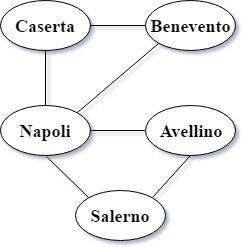
\includegraphics[scale=0.7]{ConstraintGraph.jpg}
		\end{center}
		
		Analizziamo il caso in cui l'agente disponga di solo 2 colori.
		\begin{lstlisting}
Dominio = {Colore1, Colore2}
		\end{lstlisting}
		Applicando il \texttt{Backtracking Search} si perviene presto alla conclusione dell'impossibilità di risolvere il problema vincolato. Ad esempio, applicando le euristiche per migliorare l'efficienza della ricerca, assegniamo a Napoli (\texttt{Degree Heuristic}: variabile con più vincoli sulle rimanenti variabili) il valore Colore1; se procediamo assegnando Colore2 a Caserta (o qualsiasi altra variabile dato che ora presentano tutte un solo valore ammissibile), si ottiene un fallimento, poiché tramite il \texttt{Forward Checking} si osserva che Benevento non può assumere nessun valore ammissibile. Questa risultato è comune anche agli altri path dell'albero di ricerca e tutto ciò è intuitivamente comprensibile poiché con soli 2 colori non siamo in grado di soddisfare i loop di 3 nodi presenti nel grafo dei vincoli.\par
		Analizziamo il caso in cui l'agente disponga di 3 colori.
		\begin{lstlisting}
Dominio = {Colore1, Colore2, Colore3}
		\end{lstlisting}
		Proviamo un approccio differente, iniziamo ad assegnare colori alle province e poi scegliamo quella con il numero minimo di scelte possibili \texttt{Minimum remaining values}.Partiamo da Napoli e le assegniamo il Colore1,notiamo che questa scelta ha ridotto tutte le scelte rimanenti per le altre province a due, allora coloriamo Caserta con il Colore2 ora Benevento è la nostra prossima scelte perché le può essere assegnata solo un colore invece per le restanti due province ancora due, quindi Benevento avrà Colore3, Avellino di conseguenza Colore2 e Salerno Colore 3, quindi possiamo affermare che è possibile soddisfare i vincoli.\par
		Anche il caso con quattro colori sicuramente permetterà di soddisfare i vincoli, perché si è aumentato il numero di valori ammissibili rimando invariate le informazioni iniziali, comunque verifichiamo che sia così.
		\begin{lstlisting}
Dominio = {Colore1, Colore2, Colore3, Colore4}
		\end{lstlisting}
		Cambiamo euristica è scegliamo la \texttt{Least constraining value}, in questo caso andiamo a scegliere come variabile successiva quella che minimizza il numero di vincoli ammissibile per le altre. La prima che andiamo a colorare è la Campania assegnandole il Colore1,perché così facendo riduciamo tutti i colori possibili per le altre province, avendo la Campania il maggior numero di vincoli, Avellino sarà la nostra prossima scelta permettendo di diminuire il numero di valori per Salerno e Benevento, assegnandole il Colore2, poi possiamo a Benevento che riduce i colori di Caserta a 2, colorandola con il Colore3, dopodiché possiamo dare a Caserta il Colore2 e Salerno il Colore3.\par
		Come si può vedere l' aggiunta di un nuovo elemento nel Dominio,non alterando i vincoli, permette comunque la risoluzione del problema, evitando anche di utilizzare il nuovo valore, quindi possiamo affermare che con un determinato grafo dei vincoli, una volta trovata la soluzione con un determinato numero di valori,questa si trova anche se il Dominio diventa più grande, con la differenza di "elasticizzare" i vincoli, nel senso che se con tre elementi nel Dominio il numero di soluzioni possibili, sicuramente sarà molto più limitato rispetto a quello con quattro elementi, avendo molte più possibilità di scelta, potendo dire che le soluzioni che si trovano con il Dominio "allargato" racchiudono quelle del Dominio più compatto. 
	\section{Esercizio 4}
		\label{sec:es4}
		Un approccio possibile per trovare la soluzione con l' ausilio di algoritmi genetici potrebbe essere questo:
		Definire come funzione di costo il numero di conflitti, province confinanti con lo stesso colore, il nostro obiettivo è quindi quello di minimizzare questo valore.La popolazione iniziale sarà costituita da delle cartine colorate in modo casuale,dopodiché definiamo una probabilità di mutazione,se non siamo in quest' ultimo caso allora avverrà l' operazione di crossover che consiste nel prendere in modo casuale dall' elite due elementi e scegliere probabilisticamente, quanti cromosomi(province) di uno unire con i restanti dell' altro,altrimenti per la mutazione invece basterà scegliere un elemento dalla cartina e cambiarli colore a scelta tra gli altri tre, escludendo ovviamente quello già assegnato. 
		
	\end{titlepage}
\end{document}        
